\subsection{Lightcurve}

Time series data and analyses are a fundamental aspect of solar physics for which many data sources are available. In recognition of this fact, SunPy provides a \textit{Lightcurve} object designed to provide a convenient and consistent interface for handling solar time series data. The main engine behind the \textit{Lightcurve} object is the \textit{pandas} data analysis library. This library contains a large amount of functionality for manipulating and analysing time series data, making it an ideal basis for \textit{Lightcurve}.  Like all other SunPy objects, \textit{Lightcurve} is a wrapper around a data object, which in this case is the \textit{pandas} object. 

Currently, the \textit{Lightcurve} object is compatible with the following data sources; the GOES X-ray Sensor (XRS), the SDO EUV Variability Experiment (EVE), and PROBA2/LYRA. For each of these instruments, a sub-class of the \textit{Lightcurve} object is initialized (e.g. \textit{GOESLightCurve, LYRALightCurve}) which inherits from \textit{Lightcurve} but allows instrument-specific functionality to be included. Future developments will introduce support for additional instruments and data products. 
Since time series data is generally relatively small and there is no established standard as to how it should be stored and distributed, each SunPy \textit{Lightcurve} object provides the ability to download its own data in its constructor.

\subsubsection{Creating and using Lightcurves}

A \textit{Lightcurve} object may be created using a range of different methods. 
Firstly, a \textit{Lightcurve} may be created for a specific instrument based 
on an input time range (see Listing \ref{goes_lc_code} below). In this example, 
the Lightcurve constructor searches remote sites for the GOES X-ray data 
specified by the time interval, downloads the required files and subsequently 
creates the object (see also Listing \ref{goes_lc_code}).

\begin{listing}[H]
\begin{minted}{python}
>>> from sunpy import lightcurve
>>> goes=lightcurve.GOESLightCurve.create('2011-06-07 06:00',
'2011-06-07 08:00')
>>> goes.peek()
\end{minted}
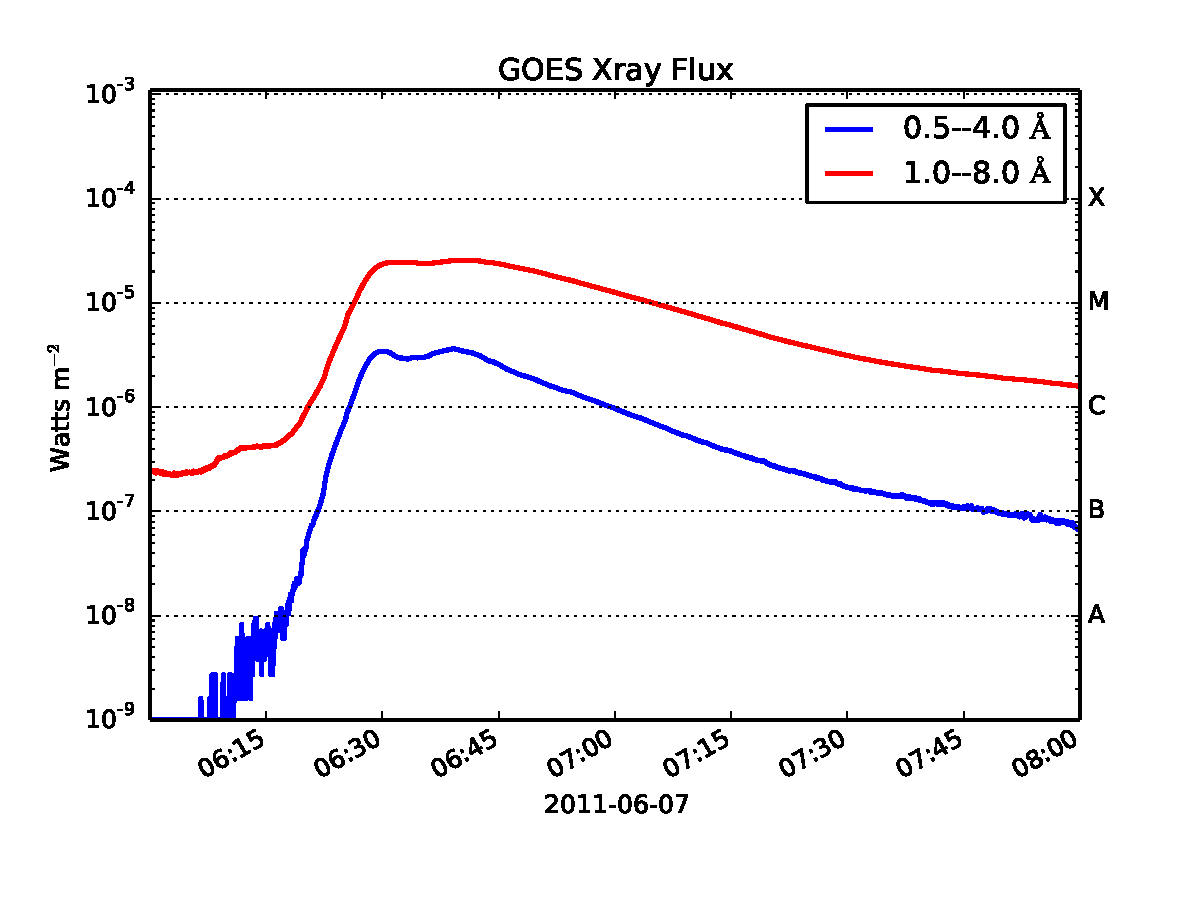
\includegraphics[width=14cm]{goes_lightcurve.pdf}
\label{goes_lc_code}
\caption{Creating a GOES lightcurve for the time interval 06:00 - 08:00 UT on 
2011 June 7 using a time range, and the result of the \texttt{peek()} command.}
\end{listing}

Alternatively, if the data file already exists on the local system, the 
\textit{Lightcurve} object may instead be initialized using that file as input 
(see Listing \ref{lyra_lc_code}).

\begin{listing}[H]
\begin{minted}{python}
>>> from sunpy import lightcurve
>>> file='lyra_20110607-000000_lev2_std.fits'
>>> lyra=lightcurve.LYRALightCurve.create(file)
>>> lyra.peek()
\end{minted}
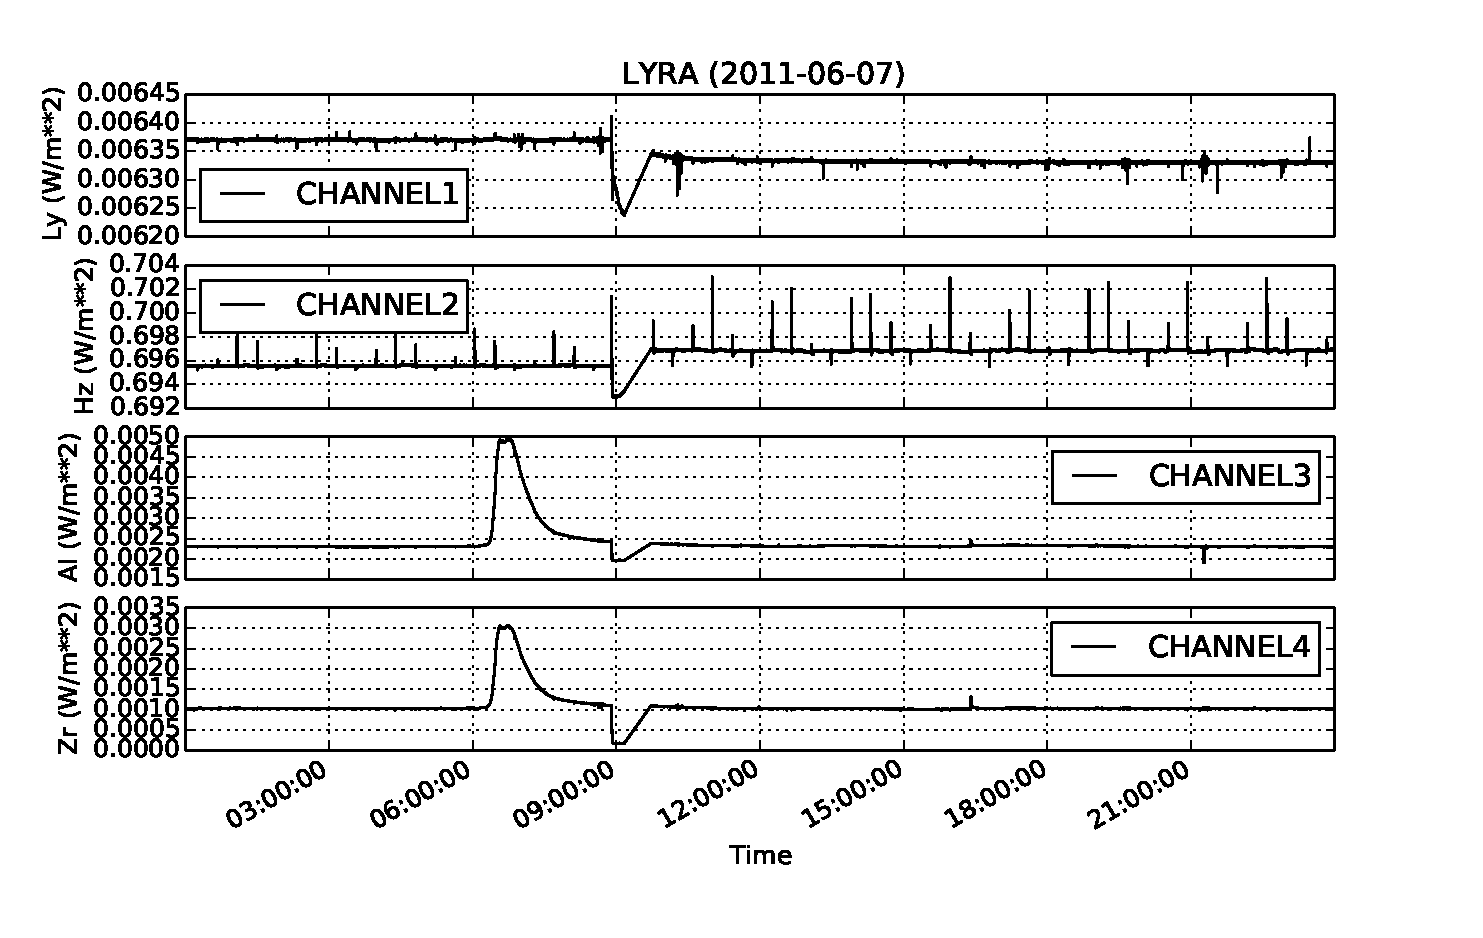
\includegraphics[width=14cm]{lyra_lightcurve.pdf}
\label{lyra_lc_code}
\caption{Creating a LYRA lightcurve for the full day of 2011 June 7 using an 
existing data file, and the result of the \texttt{peek()} command}
\end{listing}

Once the \textit{Lightcurve} has been created it may be manipulated in a variety of ways in order to perform time series analysis. Continuing from the above, we show a few simple examples of using a LYRA lightcurve. 

In the above case (Listing \ref{lyra_lc_code}), we created a LYRA Lightcurve spanning the full day of 2011 June 7. To extract the sub-interval 06:00 - 07:00 UT into a new \textit{Lightcurve} called \verb|lyra_zoom| we simply do the following:

\begin{listing}[H]
\begin{minted}{python}
>>> from sunpy.time import TimeRange
>>> tran=TimeRange('2011-06-07 06:00','2011-06-07 07:00')
>>> lyra_zoom = lyra.truncate(tran)
\end{minted}
\label{lyra_truncate}
\caption{Extracting a sub-interval from a Lightcurve.}
\end{listing}

Also in the example shown in Listing \ref{lyra_lc_code}, direct access to the data and time information in the object is available through \verb|lyra.data| and \verb|lyra.data.index| respectively.

\begin{listing}[H]
\begin{minted}{python}
>>> print lyra.data
<class pandas.core.frame.DataFrame>
DatetimeIndex: 1496629 entries, 2011-01-28 00:00:00.110000 to 
2011-01-28 23:59:59.983993
Data columns (total 4 columns):
CHANNEL1    1496629  non-null values
CHANNEL2    1496629  non-null values
CHANNEL3    1496629  non-null values
CHANNEL4    1496629  non-null values
dtypes: float64(4)

>>> print lyra.data.index
<class pandas.tseries.index.DatetimeIndex>
[2011-01-28 00:00:00.110000, ..., 2011-01-28 23:59:59.983993]
Length: 1496629, Freq: None, Timezone: None
\end{minted}
\label{lyra_pandas}
\caption{Accessing the data and time axis in a Lightcurve}
\end{listing}

